\documentclass{article}

\usepackage{graphicx}
\usepackage{amsmath}
\usepackage{siunitx}
\usepackage{placeins}

\usepackage[margin=1in]{geometry}
\usepackage{float}


\def\hwtitle{Computational Physics HW7}
\def\hwauthor{Ethan Rooney}
\def\hwdate{2020-04-01}

\usepackage{fancyhdr}
\lhead{\hwauthor}
\chead{\hwtitle}
\rhead{\hwdate}
\lfoot{\hwauthor}
\cfoot{}
\rfoot{\thepage}
\renewcommand{\footrulewidth}{0.4pt}
\pagestyle{fancy}

\author{\hwauthor}
\title{\hwtitle}
\date{\hwdate}

\begin{document}

\maketitle
\thispagestyle{fancy}

\section{Introduction}

In this assignment we simulate a small system of particles in a Metropolis gas scenario.

\section{Results}

\subsection{Question 1}

Seen below are snapshots of 2 different systems with similar starting configurations, but different initial temperature. 
The lower energy system would correspond to something akin to a droplet of water. Some molecules have enough energy to escape the system i.e. evaporate, while the high energy system is like that of a gas where every molecule is energetic enough to turn to steam.

\begin{figure}[!htb]
	\begin{center}
		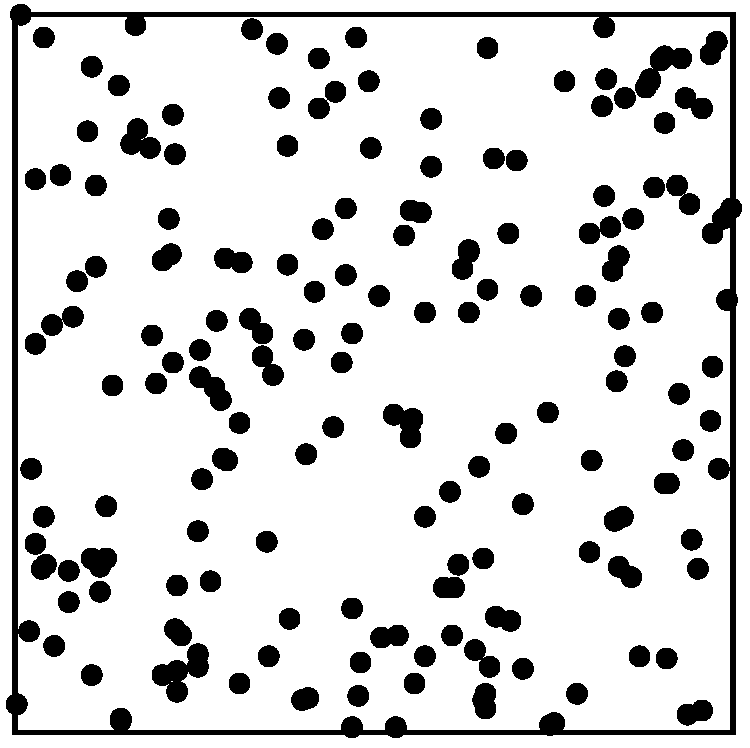
\includegraphics[width=0.6\textwidth]{5kt_thermalized.pdf}
	\end{center}
	\caption{A system of 200 molecules where initially $kT = 5$: The system is almost immediately scattered and thermalized.}
\label{fig:qual}
\end{figure}
\FloatBarrier

\begin{figure}[!htb]
	\begin{center}
		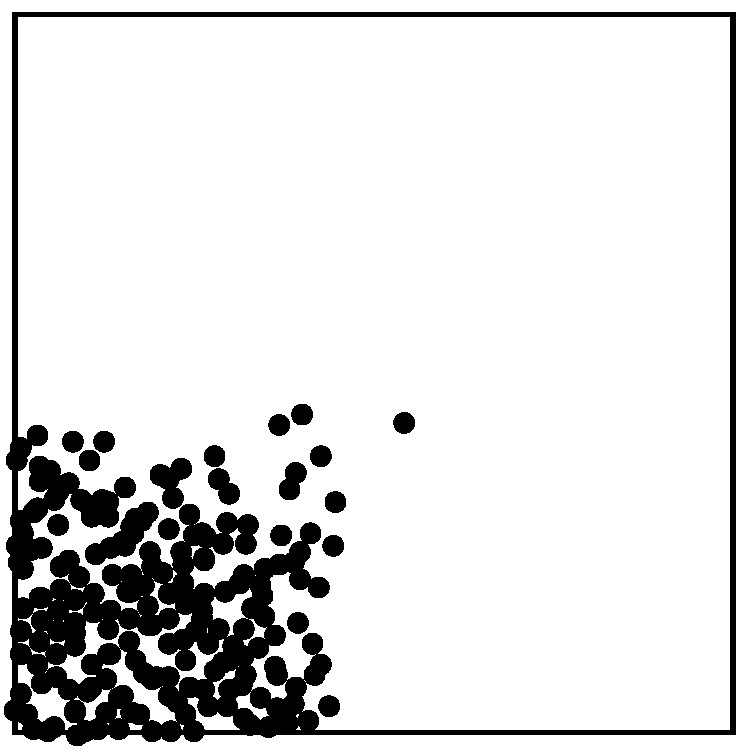
\includegraphics[width=0.6\textwidth]{05kT_thermalized.pdf}
	\end{center}
	\caption{A system of 200 molecules where initially $kT = 0.5$: The system remains condensed into a single block.}
\label{fig:qual}
\end{figure}
\FloatBarrier

For $kT = 5$: $dx = 20$ and $dv = 4$. This system is a high energy gas.

For $kT = 5$: $dx = 0.155$ and $dv = 1.3$. This system is a condensed liquid.

\subsection{Question 2}



\subsection{Question 3}


\section{Conclusion}

Should have started this assignment earlier\ldots

\end{document}

